\section{LSM9DS1}
Der benyttes en IC (LSM9DS1), som både indeholder magnometer, gyroskop og accelerometer, hvor der benyttes accelerometeret og gyroskopet. Det er muligt at indstille accelerometeret til $\pm$1, 4, 8 eller 16 g, og gyroskopet kan måle $\pm$245, 500 eller 2000 grader per sekund.\citep{Jimb02016} \newline
LSM9DS1 har ni frihedsgrader, hvormed det måler i x-, y- og z-aksen for både magnometeret, gyroskopet og accelerometeret, hvilket kan ses på \figref{vores_IC}. Akserne for gyroskopet og accelerometeret internt følger højrehåndsreglen.\citep{Jimb02016}\newline
Accelerometeret og gyroskopet bruger ikke lige meget strøm, accelerometeret bruger 600$\textmu$A, mens gyroskopet bruger 4mA. Denne store forskel i forbrug medfører at gyroskopet kun skal tændes når der skal detekteres cykling. 

\begin{figure}[H]
	\centering
	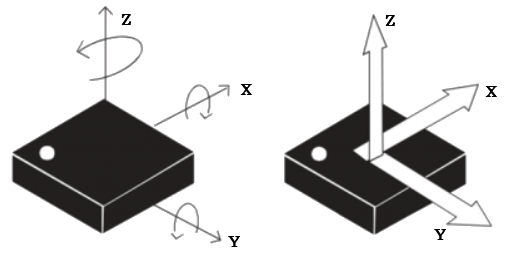
\includegraphics[scale=0.6]{figures/cDesign/LSM9DS1.png}
	\caption{På figuren ses akserne fra IC'en LSM9DS1, hvor magnometerets (til venstre) akse i realiteten er flippet i forhold til gyroskopet (i midten) og accelerometeret (til højre).\citep{Jimb02016}}
	\label{vores_IC}
\end{figure}

Accelerometeret kan både bruges med en SPI og en I$^{2}$C, og mikrocontrolleren har begge dele. Der ønskes at benytte I$^{2}$C funktionen, da der både skal sendes data, men også modtages data om hvorvidt gyroskopet skal tændes eller slukkes. For at benytte punktionen sættes pinnen CS\_AG sættes høj, og de fire pinne SDO og CS benyttes ikke. 

, da der ønskes at benytte  Alle pins kan ses på \figref{IC_pins}

\begin{figure}[H]
	\centering
	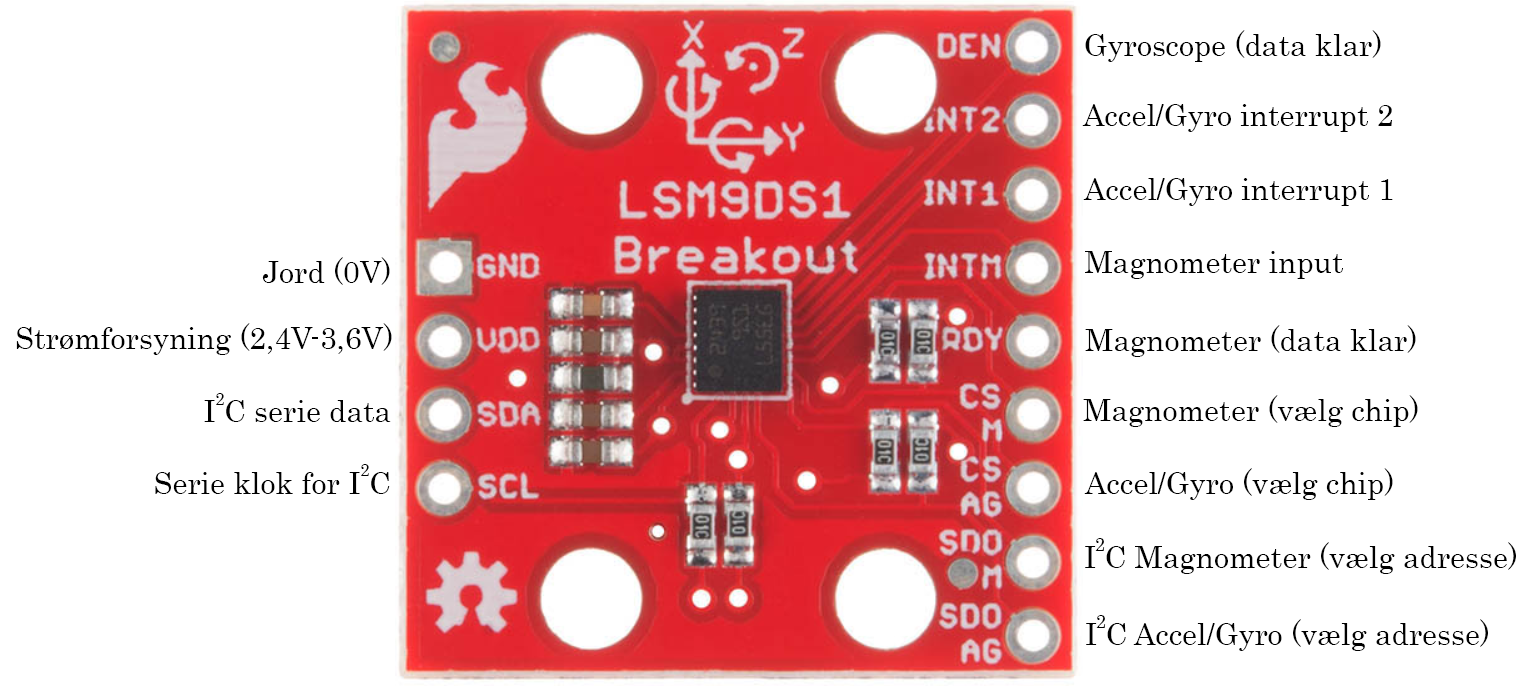
\includegraphics[scale=0.35]{figures/cDesign/accelerometeret.png}
	\caption{På figuren ses Udgangene fra IC'en.\citep{Jimb02016}}
	\label{IC_pins}
\end{figure}

